% -*- coding: utf-8 -*-
\errorcontextlines=200
\documentclass[11pt,dvipdfmx,b5paper]{book}

\usepackage{times}
\usepackage{courier}
\usepackage{comment}
\usepackage{subfig}
\usepackage{graphicx}

\usepackage{enumitem}
\usepackage{url}
\usepackage{listings}
\usepackage{tikz} % Drawing sliding-tile
\usepackage{xcolor}

%%%%%%%%%%%%%%%%%%%%%
% Math
\usepackage{amsmath}
\usepackage{amsthm}
\usepackage{amssymb}
\usepackage{mathtools}
\DeclarePairedDelimiter\ceil{\lceil}{\rceil}
\DeclarePairedDelimiter\floor{\lfloor}{\rfloor}

%%%%%%%%%%%%%%%%%%%%%
% Format
\usepackage[Bjornstrup]{fncychap}
\usepackage{titlesec}
\usepackage[framemethod=TikZ]{mdframed}
\usepackage{booktabs}

\setcounter{secnumdepth}{3}
\renewcommand{\baselinestretch}{1.15}

\usepackage{appendix}
\usepackage{hyperref}
\usepackage{makeidx}
\makeindex


%%%%%%%%%%%%%%%%%%%%
% Algorithm
\usepackage[boxruled,linesnumbered,noend]{algorithm2e}
\SetKwInOut{Input}{Input}
\SetKwInOut{Output}{Output}
\SetKwInOut{Side}{Side effect}
\SetKwComment{Comment}{$\triangleright$}{}

\begin{document}


% \begin{figure}
%   \begin{tikzpicture}[scale=0.5]
%     % MDP i
\node [draw, circle, minimum size=0.7cm] (a) at (2, 2) {$a$};
\node [draw, circle, minimum size=0.7cm] (b) at (4, 2) {$b$};
\node [draw, circle, minimum size=0.7cm] (c) at (0, 4) {$c$};
\node [draw, circle, minimum size=0.7cm] (d) at (0, 2) {$d$};
\node [draw, circle, minimum size=0.7cm] (e) at (2, 0) {$e$};
\node [draw, circle, minimum size=0.7cm] (f) at (4, 0) {$f$};
\node [draw, circle, minimum size=0.7cm] (g) at (0, 0) {$g$};
\node [draw, circle, minimum size=0.5cm] at (0, 0) {};

\coordinate[above of=a] (init);

\draw[->] (init) -- (a);
\draw[-] (a) -- (b);
\draw[-] (a) -- (c);
\draw[-] (a) -- (d);
\draw[-] (b) -- (e);
\draw[-] (b) -- (f);
\draw[-] (c) -- (d);
\draw[-] (d) -- (g);
\draw[-] (e) -- (f);
\draw[-] (d) -- (g);

%   \end{tikzpicture}
% \end{figure}
% 
% \begin{figure}
%   \begin{tikzpicture}[scale=0.5]
%     % MDP i
\node (a0) at (4, 6) {$a$};

\node (b1) at (2, 4) {$b$};
\node (c1) at (4, 4) {$c$};
\node (d1) at (6, 4) {$d$};

\node (e2) at (0, 2) {$e$};
\node (f2) at (2, 2) {$f$};
\node (d2) at (4, 2) {$d$};
\node (c2) at (6, 2) {$c$};
\node (g2) at (8, 2) {$g$};

\node (f3) at (0, 0) {$f$};
\node (e3) at (2, 0) {$e$};
\node (a31) at (3, 0) {$a$};
\node (c3) at (4, 0) {$c$};
\node (g3) at (5, 0) {$g$};
\node (a32) at (6, 0) {$a$};

\draw[-] (a0) -- (b1);
\draw[-] (a0) -- (c1);
\draw[-] (a0) -- (d1);
\draw[-] (b1) -- (e2);
\draw[-] (b1) -- (f2);
\draw[-] (c1) -- (d2);
\draw[-] (d1) -- (g2);
\draw[-] (d1) -- (c2);
\draw[-] (e2) -- (f3);
\draw[-] (f2) -- (e3);
\draw[-] (d2) -- (a31);
\draw[-] (d2) -- (c3);
\draw[-] (d2) -- (g3);
\draw[-] (c2) -- (a32);

%   \end{tikzpicture}
% \end{figure}

% \begin{figure}
%   \begin{tikzpicture}[scale=0.5]
%     % Grid pathfinding

\foreach \x in {0,...,3}
  \foreach \y in {0,...,3}
    {\node [draw, circle, fill=black] (\x\y) at (1.5*\x, 1.5*\y) {};}

\foreach \x in {0,...,3}
  \foreach \y in {0,...,2}
           {\draw (1.5 * \x, 1.5 * \y) -- (1.5 * \x, 1.5 * \y + 1.5);}

\foreach \y in {0,...,3}
  \foreach \x in {0,...,2}
           {\draw (1.5 * \x, 1.5 * \y) -- (1.5 * \x + 1.5, 1.5 * \y);}
           
\foreach \x in {0,...,3}
         {\node at (1.5 * \x, -1) {\x};
          \node at (-1, 1.5 * \x) {\x};
         }

%   \end{tikzpicture}
% \end{figure}

% \begin{figure}
%   \begin{tikzpicture}[scale=0.5]
%     % Sliding tile puzzle

\draw (0, 0) grid (4, 4);

\foreach \x in {0,...,3}
  \foreach \y in {0,...,3}
  {
        \pgfmathsetmacro{\val}{int(\x+3*\y+1)}
        \ifthenelse{\x=3 \AND \y=3}{;}{
          \node at (\x + 0.5, 3 - \y + 0.5) {\val};
        }
  }

\draw[fill=gray] (3,0) rectangle (4, 1);

%   \end{tikzpicture}
% \end{figure}

% \begin{figure}
%   \texttt{Sequence1 -TCA----\\
Sequence2 ATCACG--\\
Sequence3 ATGAGG--\\
Sequence4 ---AGGCA

}
% \end{figure}

\begin{figure}
  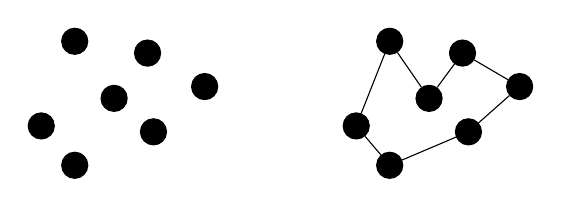
\begin{tikzpicture}[scale=0.5]
    \foreach \x in {0, 8}
  {
    \pgfmathsetmacro{\noise}{0.15}           
\node[draw,circle,fill=black] (1\x) at (\x+0, 0) {};
\node[draw,circle,fill=black] (2\x) at (\x+2, 1-\noise) {};
\node[draw,circle,fill=black] (3\x) at (\x+3+2*\noise, 2) {};
\node[draw,circle,fill=black] (4\x) at (\x+2-\noise, 3-\noise) {};
\node[draw,circle,fill=black] (5\x) at (\x+1, 2-2*\noise) {};
\node[draw,circle,fill=black] (6\x) at (\x+0, 3+\noise) {};
\node[draw,circle,fill=black] (7\x) at (\x-1+\noise, 1) {};
}

\foreach \a in {1,...,6}
  {
    \pgfmathsetmacro{\n}{int(\a+1)}
    \draw[-] (\a8) -- (\n8);
  }

\draw[-] (78) -- (18);

  \end{tikzpicture}
\end{figure}

\end{document}
